\documentclass[]{standalone}
\usepackage{tikz}
\usepackage{siunitx}
\usetikzlibrary{scopes, patterns,arrows, decorations.markings}
\definecolor{copper}{rgb}{0.85, 0.54, 0.4}

\begin{document}
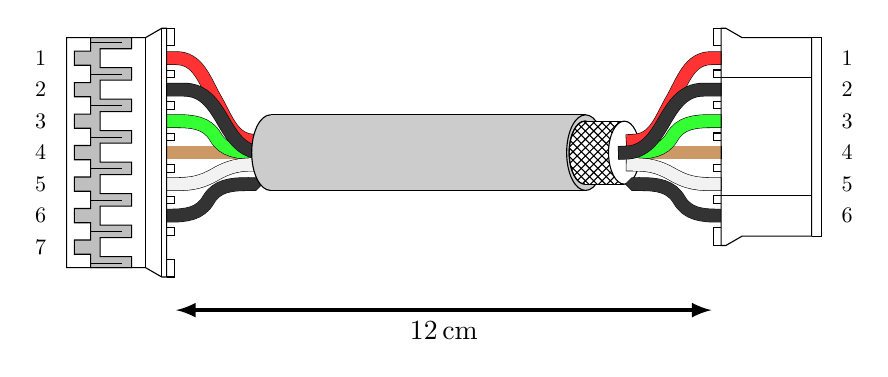
\begin{tikzpicture}[x=1mm, y=1mm, scale=2, transform shape]
    \def\cylinder#1#2#3#4#5{
        % #1 diameter
        % #2 length
        % #3 color
        % #4 pattern
        % #5 label
        \draw[fill=#3, #5]%
            (-#2,0) ellipse (#1/4 and #1/2)%
        ;%
        \draw[#4, #5]%
            (-#2,0) ellipse (#1/4 and #1/2)%
        ;%
        \fill[#3]%
            (-#2,#1/2) rectangle (0,-#1/2)%
        ;% background
        \fill[#4]%
            (-#2,#1/2) rectangle (0,-#1/2)%
        ;%
        \draw[fill=#3, #5]%
            (0,0) ellipse (#1/4 and #1/2)%
        ;%
        \draw[#5]%
            (0,#1/2) --    +(-#2,0)%
            (0,-#1/2) -- +(-#2,0)%
        ;%
    }
  
    \def\wire#1#2#3#4#5{
        % #1 color
        % #2 length
        % #3 height
        % #4 x shift
        % #5 angle
        % If we must have rounded caps, check out:
        % https://tex.stackexchange.com/questions/21392/rounded-ends-with-tikz
        \draw[very thin, double distance = 0.8mm*2, double=#1, line cap=rect]%
            (0mm,0mm) to[out=0, in=#5-180] ++(#2/2,#3/2) to[out=#5, in=180] ++(#2/2,#3/2) -- ++(#4,0) -- ++(0.2mm,0)%
        ;
    }

    \def\wireWithTip#1#2#3#4#5{
        % #1 color
        % #2 length
        % #3 height
        % #4 x shift
        % #5 angle
        \draw[very thin, double distance = 0.8mm*2, double=#1, triangle 90 cap-, postaction={draw,color=#1, line width=0.8mm*2, shorten <=.1mm}]%
            (-1mm,0mm) -- (0mm,0mm) to[out=0, in=#5-180] ++(#2/2,#3/2) to[out=#5, in=180] ++(#2/2,#3/2) -- ++(#4,0) -- ++(0.2mm,0)%
        ;%
        %\draw[very thin, fill=#1] (-0.4mm-0.1pt, 0.4mm+0.09pt) -- ++(-0.1pt,0) -- (-1.6mm,0) -- (-0.4mm-0.2pt, -0.4mm-0.09pt) -- ++(0.1pt,0);
    }

    \def\PHRTop#1{%
        % #1 Number of pins
        \begin{scope}[xshift=-#1*1mm-0.9mm, yshift=3.425mm]
            \draw%
                (0,-0.5) -- ++(0,0.5) -- ++(1.125,0) -- ++(0,-0.5)%
            ;
            \draw%
                (0.675 + #1*2,-0.5) -- ++(0,0.5) -- ++(1.125,0) -- ++(0,-0.5)%
            ;
            \foreach \i in {1,...,\numexpr #1-1}
            {
                \draw (0.675 + \i*2,-0.5) -- ++(0,0.5) -- ++(0.475,0) -- ++(0,-0.5);
            }
            % pin lables
            \foreach \i in {1,..., #1} {
                \node[rotate=-90, scale=0.4] at (#1*2+1.9-\i*2,-8.5) {\i};
            }
            \draw%
                (0, -0.5) -- ++(0,-0.3) -- ++(0.6, -1.039) -- ++(0,-4.411) -- ++(#1*2+0.6,0) -- ++(0,4.411) -- ++(0.6, 1.039) -- ++(0,0.3) -- cycle%
            ;
            \draw%
                (0.6,-6.25) -- ++(0,-0.6) -- ++(#1*2+0.6,0) -- ++(0,0.6)%
            ;
            \draw%
                (3.15,-0.5) -- ++(0,-5.75) (3.15+-4.5+#1*2,-0.5) -- ++(0,-5.75)%
            ;
        \end{scope}
    }

    \def\PHRBottom#1{%
    % #1 Number of pins
        \begin{scope}[xshift=-#1*1mm-0.9mm, yshift=3.425mm]
            \draw%
                (0,-0.5) -- ++(0,0.5) -- ++(1.125,0) -- ++(0,-0.5)%
            ;
            \draw%
                (0.675 + #1*2,-0.5) -- ++(0,0.5) -- ++(1.125,0) -- ++(0,-0.5)%
            ;
            \foreach \i in {1,...,\numexpr #1-1}
            {
                \draw (0.675 + \i*2,-0.5) -- ++(0,0.5) -- ++(0.475,0) -- ++(0,-0.5);
            }
            % pin lables
            \foreach \i in {1,..., #1} {
                \node[rotate=90, scale=0.4] at (-0.1+\i*2,-8.5) {\i};
            }
            \draw%
                (0, -0.5) -- ++(0,-0.3) -- ++(0.6, -1.039) -- ++(0,-5.011) -- ++(#1*2+0.6,0) -- ++(0,5.011) -- ++(0.6, 1.039) -- ++(0,0.3) -- cycle%
            ;
            \draw%
                (0, -0.8) -- ++(1.8 + #1*2,0)%
            ;
            \draw%
                (0.6, -1.839) -- ++(0.6 + #1*2,0)%
            ;
            \draw[fill=lightgray]%
                (0.6, -2.72)%
                \foreach \i in {1,..., #1} {
                    -- (0.9 + \i*2 - 2, -2.72) -- ++(0.4,0) -- ++(0, -2) -- ++(1.2,0) -- ++(0, 2) -- ++(0.4,0)
                }%
                -- ++(0.3,0) -- (1.2 + #1*2, -5.32) -- ++(-0.3,0)%
                \foreach \i in {1,..., #1} {
                    -- ++(-0.55,0) -- ++(0, -1.03) -- ++(-0.9,0) -- ++(0, 1.03) -- ++(-0.55,0)
                }%
                -- ++(-0.3,0)%
                -- cycle%
            ;
            \foreach \i in {0,..., #1} {
                \draw[ultra thin] (0.9 + \i*2, -5.32) -- ++ (0,++2);
            }
        \end{scope}
    }

    % Wires left
    \begin{scope}[xshift=-2.5mm-18mm, yshift=0mm, xscale=-1]
        \wire{brown!80}{5mm}{0mm}{0.5mm}{0}
    \end{scope}
    \begin{scope}[xshift=-3mm-18mm, yshift=0.75mm, xscale=-1]
        \wire{red!80}{5mm}{5.25mm}{0}{60}
    \end{scope}
    \begin{scope}[xshift=-3mm-18mm, yshift=0mm, xscale=-1]
        \wire{green!80}{5mm}{2mm}{0mm}{60}
    \end{scope}
    \begin{scope}[xshift=-3mm-18mm, yshift=-0.75mm, xscale=-1]
        \wire{lightgray!20}{5mm}{-1.25mm}{0mm}{-30}
    \end{scope}
    \begin{scope}[xshift=-2.5mm-18mm, yshift=0mm, xscale=-1]
        \wire{black!80}{5mm}{4mm}{0.5mm}{60}
    \end{scope}
    \begin{scope}[xshift=-3.5mm-18mm, yshift=-2mm, xscale=-1]
        \wireWithTip{black!80}{4.9mm}{-2mm}{0mm}{-60}
    \end{scope}

    % Cable
    \cylinder{4.8mm}{20mm}{black!20}{shade,shading angle=180, middle color=black!10,opacity=0}{}
    \begin{scope}[xshift=7]
        \cylinder{4mm}{2.5mm}{white}{pattern=crosshatch}{}
    \end{scope}
    %\node[] at (-10mm,6mm) {Belden 9535};

    % Wires right
    \begin{scope}[xshift=2.5mm, yshift=0mm]
        \wire{brown!80}{5mm}{0mm}{0.5mm}{0}
    \end{scope}
    \begin{scope}[xshift=3mm, yshift=0.75mm]
        \wire{red!80}{5mm}{5.25mm}{0}{60}
    \end{scope}
    \begin{scope}[xshift=3mm, yshift=0mm]
        \wire{green!80}{5mm}{2mm}{0mm}{60}
    \end{scope}
    \begin{scope}[xshift=3mm, yshift=-0.75mm]
        \wire{lightgray!20}{5mm}{-1.25mm}{0mm}{-30}
    \end{scope}
    \begin{scope}[xshift=2.5mm, yshift=0mm]
        \wire{black!80}{5mm}{4mm}{0.5mm}{60}
    \end{scope}
    \begin{scope}[xshift=3.5mm, yshift=-2mm]
        \wireWithTip{black!80}{4.9mm}{-2mm}{0mm}{-60}
    \end{scope}

    \begin{scope}[xshift=11.53mm, yshift=1mm, rotate=90]
        \PHRTop{6}
    \end{scope}
    \begin{scope}[xshift=-29.53mm, yshift=0mm, rotate=-90]
        \PHRBottom{7}
    \end{scope}

    \draw
        (-26mm, -10mm) edge[latex-latex,line width=0.5mm] node[below,  scale=0.5] {\qty{12}{\cm}} (8mm, -10mm)
    ;
\end{tikzpicture}

\end{document}
